\documentclass{beamer}
\usetheme{Berkeley}

\begin{document}

\title[Python] % (optional, only for long titles)
{Data Mining with Python}
\subtitle{Most of the work is in preparing the data}
\author{Clark Fitzgerald}
\institute{Cisco Systems}
\date{Winter 2014} % (optional)
\subject{Statistics}


\frame{\titlepage}

%%%%%%%%%%%%%%%%%%%%%%%%%%%%%%%%%%%%%%%%%%%%%%%%%%%%%%%%%%%%

\begin{frame}
\frametitle{Statisticians \emph{love} data visualizations}
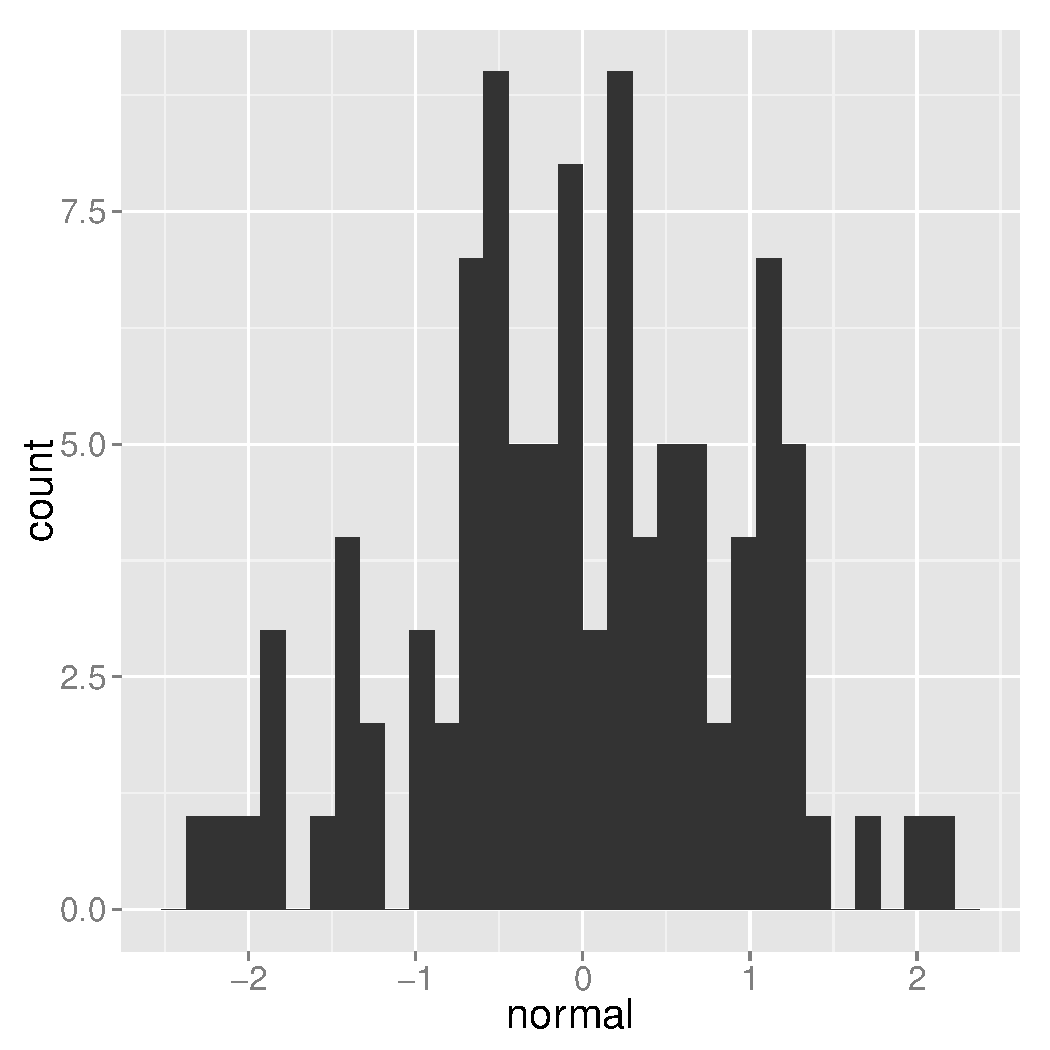
\includegraphics[height=2.5in]{figs/normal.pdf}
\end{frame}

%%%%%%%%%%%%%%%%%%%%%%%%%%%%%%%%%%%%%%%%%%%%%%%%%%%%%%%%%%%%

\begin{frame}
\frametitle{This is the second slide}
Here is where I would write a bunch of text. Visit the \href{https://github.com/nick-ulle/2015-python-course}{course website}
    \begin{block}{Summary}
    Programming is super fun.
    \end{block}
\end{frame}

%%%%%%%%%%%%%%%%%%%%%%%%%%%%%%%%%%%%%%%%%%%%%%%%%%%%%%%%%%%%

\begin{frame}
\frametitle{Powerpoints should always contain $n$ bullet points}

\begin{itemize}
\item Bullet 1
\item Bullet 2
\item ...
\item Bullet $n$
\end{itemize}

\end{frame}

%%%%%%%%%%%%%%%%%%%%%%%%%%%%%%%%%%%%%%%%%%%%%%%%%%%%%%%%%%%%

\begin{frame}
\frametitle{Makefile in progress here!}
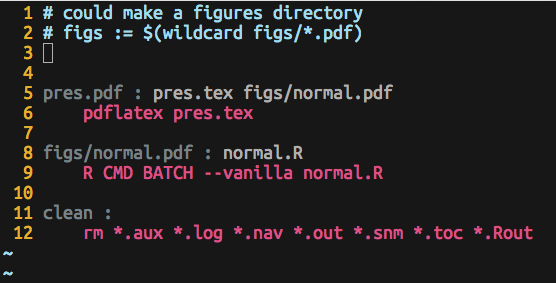
\includegraphics[width=4in]{figs/makefile.png}

This is a screenshot, a PNG file.
\end{frame}

%%%%%%%%%%%%%%%%%%%%%%%%%%%%%%%%%%%%%%%%%%%%%%%%%%%%%%%%%%%%

\begin{frame}[fragile]
\frametitle{Evolving Makefile contents}
\begin{verbatim}

pres.pdf : pres.tex figs/normal.pdf
    pdflatex pres.tex

figs/normal.pdf : normal.R
    R CMD BATCH --vanilla normal.R 

clean :
    rm *.aux *.log *.nav *.out *.snm *.toc *.Rout

\end{verbatim}
\end{frame}

%%%%%%%%%%%%%%%%%%%%%%%%%%%%%%%%%%%%%%%%%%%%%%%%%%%%%%%%%%%%

\begin{frame}[fragile]
\frametitle{Evolving Makefile contents}
\begin{verbatim}

# Everything in the `figs` directory
figs := $(wildcard figs/*)


pres.pdf : pres.tex $(figs)
    pdflatex pres.tex

\end{verbatim}

We have gained a bit of abstraction by specifying that {\tt pres.pdf} depends on everything in the {\tt figs} directory.

\end{frame}


\end{document}
